

%% ===================================================================
\section{\vrev{파레토 불확실성 환경의 C3 결과}}
\label{sec:result_c3}
%% ===================================================================

\textbf{C3} 조건은 C2의 가우시안 불확실성을 파레토 분포
($U_{\text{raw}}^{(P)} \sim 6 \cdot \mathrm{Pareto}(\alpha=3)$)로 대체한 것으로,
극단 사건(extreme events)이 $\DRTO$에 미치는 구조적 영향을
관측하는 핵심 조건이다.

\figref{fig:pareto_concept}\refpo{fig:pareto_concept}{은}{는} 가우시안과 파레토 분포의 확률밀도함수 비교 및
생존함수(survival function)를 통한 꼬리 행동의 질적 차이를 도식화한 것이다.
\chg{여기서 생존함수 $\bar{F}(u) = P(U > u) = 1 - F(u)$는 확률변수 $U$가 특정 값 $u$를 초과할 확률을
나타내며, 예컨대 $\bar{F}(10) = 0.01$이면 불확실성이 10시간을 초과할 확률이 1\%임을 의미한다. 생존함수
값이 높을수록 해당 수준 이상의 극단 사건이 빈번함을 뜻하며, 분포의 꼬리가 얼마나 느리게 감소하는지를
직접 비교할 수 있다.}
두 분포는 동일한 기대값 $E[U] = 3.0$을 공유하지만,
파레토 꼬리는 가우시안의 지수적 감쇠에 비해
극단 영역에서 현저히 높은 초과 확률을 나타낸다.
\chg{그림에서 패널 (a)는 동일 평균 $E[U] = 3.0$ 하의 확률밀도함수 비교를, 패널 (b)는 로그 스케일
생존함수 비교를 보인다. 가우시안의 지수적 감쇠($\sim e^{-x^2/2}$)에 비해 파레토 감쇠는 멱법칙($\sim x^{-3}$)을
따르며, 그 결과 P99에서 $U_{\text{raw}}$ 원시값은 가우시안 $5.326$, 파레토 $21.85$로 약 $4.1$배 차이를 보인다.}

\begin{figure}[htbp]
  \centering
  \begin{tikzpicture}
    % ── Panel (a): Gaussian vs Pareto PDF ──
    \begin{axis}[
      name=panelA,
      width=0.47\textwidth,
      height=6.5cm,
      xlabel={$U_{\text{raw}}$ (불확실성 수준, 시간)},
      ylabel={확률밀도},
      title={\textbf{(a)} 가우시안 vs.\ 파레토: 확률밀도함수 비교},
      title style={font=\small\bfseries},
      xmin=0, xmax=15,
      ymin=0, ymax=0.46,
      ymajorgrids=true,
      grid style={dashed, black},
      legend style={at={(0.98,0.88)}, anchor=north east, font=\scriptsize},
      ]
      % Gaussian N(3,1) PDF
      \addplot[blue!70!black, thick, smooth, domain=0:15, samples=120]
        {1/(sqrt(2*pi)*1)*exp(-0.5*((x-3)/1)^2)};
      \addlegendentry{Gaussian $N(3, 1)$}

      % Pareto PDF: f_Y(y) = α/(y/6+1)^(α+1) / 6, α=3
      \addplot[red!70!black, thick, smooth, domain=0.01:15, samples=120]
        {3.0 / ((x/6+1)^4) / 6.0};
      \addlegendentry{Pareto $6 \cdot \mathrm{Pareto}(3)$}

      % Mean line
      \draw[black, dashed, thick] (axis cs:3, 0) -- (axis cs:3, 0.42);
      \node[font=\scriptsize, black, fill=white, inner sep=1.5pt,
            rounded corners=1pt] at (axis cs:3, 0.44)
        {$E[U] = 3.0$h (동일 평균)};

      % Heavy tail annotation
      \node[font=\tiny, red!70!black, align=center, fill=white, inner sep=1pt,
            rounded corners=1pt] at (axis cs:11.5, 0.08)
        {중꼬리(파레토)\\멱법칙 감쇠};

      % Light tail annotation
      \node[font=\tiny, blue!70!black, align=center, fill=white, inner sep=1pt,
            rounded corners=1pt] at (axis cs:7.0, 0.16)
        {경꼬리(가우시안)\\지수적 감쇠};
    \end{axis}

    % ── Panel (b): Survival function (log scale) ──
    \begin{axis}[
      at={(panelA.east)},
      anchor=west,
      xshift=18mm,
      width=0.47\textwidth,
      height=6.5cm,
      xlabel={$U_{\text{raw}}$ (불확실성 수준, 시간)},
      ylabel={$P(U > u)$ (생존함수)},
      title={\textbf{(b)} 꼬리 행동: 생존함수 비교 (로그 스케일)},
      title style={font=\small\bfseries},
      xmin=0, xmax=20,
      ymode=log,
      ymin=1e-6, ymax=1.1,
      ymajorgrids=true,
      grid style={dashed, black},
      legend style={at={(0.98,0.98)}, anchor=north east, font=\scriptsize},
      ]
      % Gaussian survival: 1 - Phi((x-3)/1)
      % Logistic approximation: 1-Phi(z) ≈ 1/(1+exp(1.7*(x-3)))
      \addplot[blue!70!black, thick, smooth, domain=0:15, samples=150]
        {1/(1+exp(1.7*(x-3)))};
      \addlegendentry{Gaussian $N(3, 1)$}

      % Pareto survival: P(Y>y) = (1/(y/6+1))^3
      \addplot[red!70!black, thick, smooth, domain=0.01:20, samples=150]
        {(1/(x/6+1))^3};
      \addlegendentry{Pareto $6 \cdot \mathrm{Pareto}(3)$}

      % P99 line
      \draw[black, dotted, thin] (axis cs:0, 0.01) -- (axis cs:20, 0.01);
      \node[font=\tiny, black, fill=white, inner sep=1pt, anchor=east] at (axis cs:20, 0.003) {P99};

      % Fill excess tail risk
      % (visual approximation — the area where Pareto > Gaussian)
      \node[font=\tiny, red!70!black, fill=orange!10, inner sep=2pt,
            rounded corners=1pt, align=center] at (axis cs:12, 0.005)
        {초과 꼬리 위험\\(Pareto $>$ Gaussian)};
    \end{axis}
  \end{tikzpicture}
  \caption{파레토 불확실성 개념도}
  \label{fig:pareto_concept}
\end{figure}


%% -------------------------------------------------------------------
\subsection{\vrev{기술통계}}
\label{subsec:c3_descriptive}
%% -------------------------------------------------------------------

C3 조건의 효율성 비율 평균은 $\bar{\eta}_{\text{C3}} = 1.514$,
$\mathrm{SD} = 0.791$로 나타났다.
$\DRTO$ 평균은 $9.085$시간이다.
평균은 C2의 $1.682$보다 $0.168$ 낮으나,
표준편차는 C2의 $0.615$ 대비 $1.29$배로 증가하였다.
이는 파레토 분포의 특성이
평균보다는 분산과 극단값에서 현저한 차이를 만들어냄을 보여준다.

\chg{불확실성 프리미엄 비율을 보면,} 전체 표본 중 $\eta_{\text{C3}} > 1.0$인 비율은 $70.8\%$로서,
C2의 $84.9\%$보다 $14.1$\,pp 낮다.
이는 파레토 분포의 높은 분산 때문에 관측성의 하향 효과가
불확실성의 상향 효과를 상쇄하는 빈도가 C2보다 높기 때문이다.
그러나 $\eta > 1.0$인 표본들의 \textit{크기}는 C2보다 훨씬 크며,
이는 CVaR 분석에서 확인된다(\subsecref{subsec:cvar}).

\chg{효과 크기 측면에서,} C2 대비 C3의 Cohen's $d = -0.238$로서 사실상 \textbf{소효과(small effect)}에 해당한다.
이는 두 조건의 평균이 유사하기 때문이며, 파레토 효과가
평균적 수준이 아닌 극단 영역에서 작동한다는 것을 의미한다.
한편, C1 대비 C3의 Cohen's $d = +1.169$는 \textbf{대효과(large effect)}에
해당하여, 순수 관측성 조건(C1)에서 파레토 불확실성 조건(C3)으로의
전환이 $\eta$에 실질적이고 큰 변화를 야기함을 보여준다.
다만, C1 대비 C2의 $d = +1.871$과 비교하면 $0.702$만큼 낮아,
가우시안 불확실성이 평균 수준에서는 파레토보다 더 큰 효과를 산출함을 알 수 있다.
\tabref{tab:c3_effect_size}\refpo{tab:c3_effect_size}{은}{는} C3의 인접 조건 대비 효과 크기를 정리한 것이다.

\begin{table}[htbp]
  \centering
  \caption{C3 조건의 인접 조건 대비 효과 크기 (Cohen's $d$)}
  \label{tab:c3_effect_size}
  \begin{tabular}{lccl}
    \toprule
    비교 쌍 & $\Delta\bar{\eta}$ & Cohen's $d$ & 해석 \\
    \midrule
    C3 vs.\ C0 & $+0.514$ & $+0.650$ & 중효과(medium effect) \\
    C3 vs.\ C1 & $+0.661$ & $+1.169$ & 대효과(large effect) \\
    C3 vs.\ C2 & $-0.168$ & $-0.238$ & 소효과(small effect) \\
    \bottomrule
  \end{tabular}
\end{table}

C3 vs.\ C1의 대효과($d = +1.169$)와 C3 vs.\ C2의 소효과($d = -0.238$)의
대비는, 불확실성의 도입 자체가 핵심 변화 요인이며 분포 형태(가우시안 vs.\ 파레토)의
차이는 평균 수준에서는 미미하되 극단 영역에서 발현됨을 시사한다.

\chg{C1$\leq$C3 순서 준수율(\jrev{H3}-c)을 보면,} 동일 표본($i = 1, \ldots, 10{,}000$)에서 $\eta_{\text{C1},i} \leq \eta_{\text{C3},i}$인
비율\chg{,} 즉 관측성만 적용한 C1의 복구시간이 파레토 불확실성까지 반영한 C3 이하인 표본의 비율은 $100.0\%$로서,
파레토 불확실성 조건에서는 C1 대비 C3의 순서가 \textit{예외 없이} 준수된다.
이는 파레토 분포의 높은 기대값과 양의 스케일 특성에 의해,
불확실성 프리미엄이 관측성 효과를 모든 표본에서 압도하기 때문이다.
C1$\leq$C2 순서 준수율($99.87\%$)과 비교하면, 파레토의 더 큰 불확실성 규모가
예외 없는 순서를 보장하는 데 기여함을 알 수 있다.


%% -------------------------------------------------------------------
\subsection{\vrev{P85.8 CDF 교차점과 분할 회귀}}
\label{subsec:crossover}
%% -------------------------------------------------------------------

C3 조건의 핵심적 구조적 특성은 약 P85.8 지점($\eta \approx 2.42$)에서
C2의 누적분포함수(CDF)와 교차하는 것이다.
이 교차점을 기준으로 분포 수준에서
P85.8 이하 구간은 $\eta_{\text{C3}} < \eta_{\text{C2}}$인 표본이 우세하고,
P85.8 이상 구간은 $\eta_{\text{C3}} > \eta_{\text{C2}}$인 표본이 우세하여
파레토 heavy-tail 효과가 발현한다.
이는 분포 수준의 경향성이며, 개별 관측값에 항상 성립하는 것은 아니다.

\figref{fig:c2c3_cdf}\refpo{fig:c2c3_cdf}{은}{는} C2와 C3의 $\eta$ CDF를 비교하여
P85.8 CDF 교차점을 시각화한 것이다.
분할 회귀의 구조적 분리점 역시 P85.8으로, CDF 교차점과 일치한다.

\begin{figure}[htbp]
  \centering
  \begin{tikzpicture}
    \begin{axis}[
      width=0.9\textwidth,
      height=7.5cm,
      xlabel={효율성 비율 $\eta$},
      ylabel={누적 확률 $F(\eta)$},
      xmin=0.3, xmax=4.2,
      ymin=0, ymax=1.05,
      ymajorgrids=true,
      xmajorgrids=true,
      grid style={dashed, black},
      legend style={at={(0.98,0.02)}, anchor=south east, font=\small},
      legend cell align=left,
      ]
      % Core/Tail 배경 영역
      \fill[green!8] (axis cs:0.3,0) rectangle (axis cs:2.42,1.05);
      \fill[red!8] (axis cs:2.42,0) rectangle (axis cs:4.2,1.05);

      % C2: 실제 경험적 CDF (시뮬레이션 데이터)
      \addplot[blue!70!black, thick, no markers]
        table[x=eta_C2, y=F_C2] {figures/data/cdf_c2_c3.dat};
      \addlegendentry{C2 (Gaussian, $\bar{\eta}=1.682$)}

      % C3: 실제 경험적 CDF (시뮬레이션 데이터)
      \addplot[red!70!black, thick, no markers]
        table[x=eta_C3, y=F_C3] {figures/data/cdf_c2_c3.dat};
      \addlegendentry{C3 (Pareto, $\bar{\eta}=1.514$)}

      % P85.8 교차점 수평선
      \draw[black, dashed, thick] (axis cs:0.3,0.858) -- (axis cs:4.2,0.858);

      % η≈2.42 수직선 (교차점 위치)
      \draw[black, dashed, thick] (axis cs:2.42, 0) -- (axis cs:2.42, 0.858);

      % 교차점 마커
      \addplot[only marks, mark=*, mark size=3pt, black, fill=gray!15]
        coordinates {(2.42, 0.858)};

      % 교차점 통합 레이블
      \node[font=\scriptsize, align=center, fill=white, draw=black, inner sep=2pt,
            rounded corners=1pt, text=black]
        at (axis cs:1.4, 0.95) {P85.8 CDF 교차점\\$(\eta,\; F) = (2.42,\; 0.858)$};
      \draw[-{Stealth}, black, thin]
        (axis cs:1.85, 0.92) -- (axis cs:2.38, 0.862);

      % Core 영역 레이블
      \node[font=\scriptsize, text=black]
        at (axis cs:2.05, 0.45) {$\longleftarrow$ Core 영역};

      % Tail 영역 레이블
      \node[font=\scriptsize, text=black]
        at (axis cs:2.80, 0.45) {Tail 영역 $\longrightarrow$};
    \end{axis}
  \end{tikzpicture}
  \caption{C2 vs.\ C3 누적분포함수(CDF) 비교 및 P85.8 CDF 교차점}
  \label{fig:c2c3_cdf}
\end{figure}


%% -------------------------------------------------------------------
\subsection{\vrev{CVaR 분석을 통한 극단 위험 정량화}}
\label{subsec:cvar}
%% -------------------------------------------------------------------

조건부 꼬리 기대값(Conditional Value-at-Risk, CVaR)~\citep{rockafellar2000optimization}은 특정 백분위 이상의
$\eta$ 평균을 나타내는 꼬리 위험 척도로서, 평균이나 표준편차로는
포착할 수 없는 극단 영역의 위험을 정량화한다.
\chg{구체적으로 $\mathrm{CVaR}_q = E[\eta \mid \eta \geq \eta_q]$로 정의되며, $q$번째 백분위 이상에 해당하는
표본들의 조건부 평균이다. 예컨대 $\mathrm{CVaR}_{99}$는 상위 1\%($n = 10{,}000$ 중 100개) 극단값의
평균으로서, 최악의 1\% 시나리오에서 평균적으로 복구시간이 얼마나 확대되는가를 정량화한다.}
\tabref{tab:cvar_comparison}\refpo{tab:cvar_comparison}{은}{는} C2와 C3 조건에 대해 6개 수준의 CVaR을 비교한 것이며,
\figref{fig:cvar_bar}\refpo{fig:cvar_bar}{은}{는} 이를 막대 차트로 시각화한 것이다.

\begin{table}[htbp]
  \centering
  \caption{C2 vs.\ C3 조건부 꼬리 기대값(CVaR) 비교}
  \label{tab:cvar_comparison}
  \begin{tabular}{lcccc}
    \toprule
    CVaR 수준 & C2 (Gaussian) & C3 (Pareto) & $\Delta$ & 증가율 \\
    \midrule
    CVaR$_{80}$ & 2.587 & 2.866 & $+0.279$ & $+10.8\%$ \\
    CVaR$_{85}$ & 2.674 & 3.082 & $+0.408$ & $+15.3\%$ \\
    CVaR$_{90}$ & 2.778 & 3.346 & $+0.568$ & $+20.4\%$ \\
    CVaR$_{95}$ & 2.925 & 3.665 & $+0.740$ & $+25.3\%$ \\
    CVaR$_{97}$ & 3.017 & 3.808 & $+0.791$ & $+26.2\%$ \\
    CVaR$_{99}$ & 3.180 & 3.944 & $+0.764$ & $+24.0\%$ \\
    \bottomrule
  \end{tabular}
\end{table}

\begin{figure}[htbp]
  \centering
  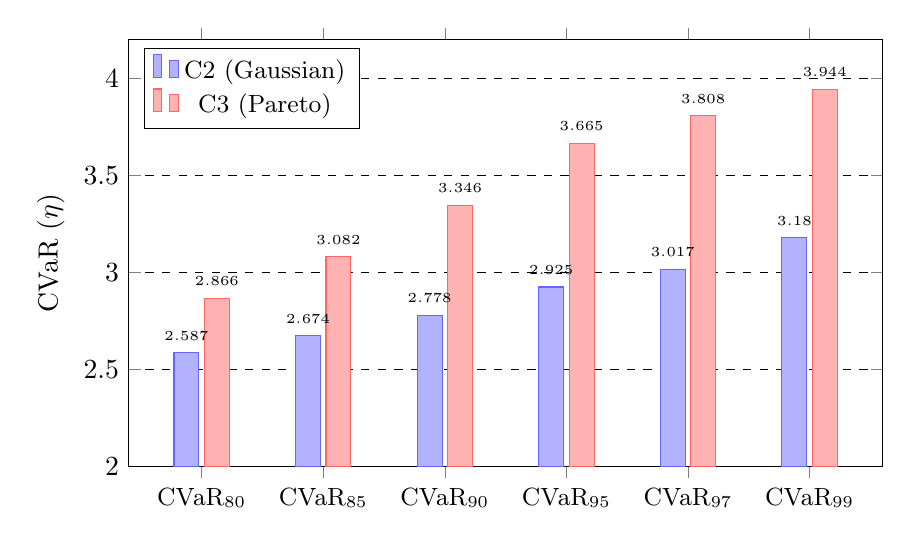
\begin{tikzpicture}
    \begin{axis}[
      ybar,
      width=0.92\textwidth,
      height=7cm,
      bar width=9pt,
      ylabel={CVaR ($\eta$)},
      symbolic x coords={CVaR$_{80}$, CVaR$_{85}$, CVaR$_{90}$, CVaR$_{95}$, CVaR$_{97}$, CVaR$_{99}$},
      xtick=data,
      xticklabel style={font=\small},
      ymin=2.0, ymax=4.2,
      ymajorgrids=true,
      grid style={dashed, black},
      nodes near coords,
      nodes near coords style={font=\tiny, above=1pt},
      every node near coord/.append style={/pgf/number format/.cd, fixed, precision=3},
      enlarge x limits=0.12,
      legend style={at={(0.02,0.98)}, anchor=north west, font=\small},
      ]
      \addplot[fill=blue!30, draw=blue!60] coordinates {
        (CVaR$_{80}$, 2.587)
        (CVaR$_{85}$, 2.674)
        (CVaR$_{90}$, 2.778)
        (CVaR$_{95}$, 2.925)
        (CVaR$_{97}$, 3.017)
        (CVaR$_{99}$, 3.180)
      };
      \addlegendentry{C2 (Gaussian)}
      \addplot[fill=red!30, draw=red!60] coordinates {
        (CVaR$_{80}$, 2.866)
        (CVaR$_{85}$, 3.082)
        (CVaR$_{90}$, 3.346)
        (CVaR$_{95}$, 3.665)
        (CVaR$_{97}$, 3.808)
        (CVaR$_{99}$, 3.944)
      };
      \addlegendentry{C3 (Pareto)}
    \end{axis}
  \end{tikzpicture}
  \caption{C2 vs.\ C3 CVaR 비교 (CVaR$_{80}$--CVaR$_{99}$)}
  \label{fig:cvar_bar}
\end{figure}

CVaR$_{80}$에서 CVaR$_{99}$로 갈수록 C3와 C2의 격차가 확대된다.
CVaR$_{80}$ 수준에서는 C3가 C2 대비 $+10.8\%$ 높으며,
CVaR$_{95}$ 수준에서는 $+25.3\%$로 약 $2.3$배 이상 확대된다.
이러한 비선형적 격차 확대는 파레토 분포의 꼬리 특성에 기인하며,
극단 사건의 빈도가 높은 산업(금융, 의료, 통신)에서 C3 조건 적용의
필요성을 직접 뒷받침한다.

\chg{CVaR 에스컬레이션 패턴을 보면,} C2의 CVaR은 $80 \to 99$ 수준에서 $2.587 \to 3.180$으로
상승하는 반면($\Delta_{80 \to 99} = 0.593$),
C3의 CVaR은 $2.866 \to 3.944$로 상위 백분위에서
더 가파르게 상승한다($\Delta_{80 \to 99} = 1.078$).
이는 C3의 극단 영역에서 $\eta$의 에스컬레이션 속도가 C2의 약 $1.8$배에
달함을 의미하며, 꼬리 위험의 구조적 비대칭성을 보여준다.

\chg{P85.8 분할 기준의 실무적 의미는 다음과 같다.} CVaR 분석 결과는 P85.8 분할 회귀 분석과 일관된다.
전체 표본의 $85.8\%$에 해당하는 Core 영역에서는 C2와 C3의 $\eta$가
거의 구분되지 않으나,
상위 $14.2\%$의 Tail 영역에서 파레토 효과가 급격히 발현한다.
이는 극단 위험 관리가 필요한 조직\chg{(}금융기관의 시장 리스크,
의료기관의 사이버 공격 대응, 통신사의 대규모 네트워크 장애 등\chg{)}에서
C3 조건의 적용이 사실상 필수적임을 시사한다.


%% -------------------------------------------------------------------
\subsection{\vrev{C2와 C3 핵심 지표 비교}}
\label{subsec:c2_c3_comparison}
%% -------------------------------------------------------------------

\tabref{tab:c2_c3_key_metrics}\refpo{tab:c2_c3_key_metrics}{은}{는} 동일 시뮬레이션 설계($n = 10{,}000$,
$\kappa = 1.2$, $R_{\max} = 24.0$h, $E[U] = 3.0$) 하에서
가우시안(C2)과 파레토(C3) 불확실성의 핵심 지표를 직접 대비한 것이다.

\begin{table}[htbp]
  \centering
  \caption{C2(가우시안) vs C3(파레토) 분포 통계 비교}
  \label{tab:c2_c3_key_metrics}
  \small
  \begin{tabular}{l rr l}
    \toprule
    \textbf{지표} & \textbf{C2 (가우시안)} & \textbf{C3 (파레토)} & \textbf{해석} \\
    \midrule
    $\bar{\eta}$          & 1.682 & 1.514 & C2가 평균적으로 높음 \\
    $\text{SD}(\eta)$     & 0.615 & 0.791 & C3가 분산 더 큼 \\
    $\eta_{\max}$         & 3.443 & 4.000 & C3가 $R_{\max}$ 포화 접근 \\
    프리미엄 비율         & 84.9\% & 70.8\% & C2가 더 빈번하게 초과 \\
    $d$ (vs C1)           & $+1.871$ & $+1.169$ & C2의 효과 크기 더 큼 \\
    순서 준수율 (C1$\leq$C$x$) & 99.87\% & 100.0\% & 양쪽 모두 높음 \\
    \bottomrule
  \end{tabular}
\end{table}
회귀분석 측면의 비교(1차/2차 $R^2$, 전진 선택, LASSO)는 4.4절에서
상세히 다룬다.

이 비교로부터 두 가지 분포 구조의 차이가 도출된다.
\textbf{첫째}, 가우시안(C2)의 대칭적 종형 분포는 평균 중심의 예측 가능한
변동을 생성하여 ``일상적 운영 변동''의 모델링에 적합하다.
\textbf{둘째}, 비대칭 파레토(C3) 분포는 극단 꼬리에서 $\eta \to 4.0$
($= R_{\max}/R_0$)에 접근하는 소수 사례를 생성하여, 꼬리 위험 탐지에서
본질적 우위를 보인다.
이러한 ``이중축'' 구조\chg{(}일상적 변동은 경꼬리(가우시안, C2) 기반으로,
극단 위험은 중꼬리(파레토, C3) 기반으로 관리\chg{)}는 \chref{ch:discussion}의
실무 적용 가이드라인에서 구체화된다.

\chg{끝으로 H3-c의 검증 결론은 다음과 같다.} \mrev{H3-c는 ``$\eta_{\text{C2}} \leq \eta_{\text{C3}}$''를 \emph{조건부}
가설로 하며, 전체 표본에서는 31.8\%에 그치나 P85.8 CDF 교차점 이상의
극단 영역에서 94.9\%가 역전된다. 조건부 명제로서 \textbf{H3-c는 채택된다}.}
